\chapter{Methodology}

\section{Evidence Chain Approach}

The core methodology is an \textbf{evidence chain}: demonstrating that a vulnerability exists, passes the verifier, and is triggered at runtime. A complete evidence chain requires validation at each compilation and execution stage, creating an unbroken lineage from source code through kernel execution that proves the vulnerability's existence and exploitability.

\subsection{Stages of the Evidence Chain}

\begin{enumerate}[label=\arabic*.]
  \item \textbf{Patch Injection}: Inject a specific ISO-IEC TS 17961-2013~\cite{ISO17961} rule violation into \texttt{xdp\_synproxy\_kern.c} via Git patch file to ensure reproducibility and version control.
  
  \item \textbf{Bytecode Inspection}: Compile the patched C code with clang/LLVM and dump the compiled eBPF object file using \texttt{llvm-objdump -d}. Confirm that the vulnerable code path is present in the bytecode and was not dead-code-eliminated by the compiler.
  
  \item \textbf{Verifier Logs}: Attempt to load the program into the kernel using \texttt{bpftool prog load -d}. Capture the verifier's approval (or rejection) and any diagnostic logs. This proves whether the verifier accepts the violation.
  
  \item \textbf{Translated Bytecode}: If the verifier accepts the program, dump the verifier's post-processing output using \texttt{bpftool prog dump xlated}. This shows the verifier-processed bytecode and confirms that the unsafe path was not eliminated by verification.
  
  \item \textbf{Runtime Trigger}: Craft PoC code (Python/Scapy or raw sockets) to execute the vulnerable code path at runtime. Send specially crafted network packets to the interface where the XDP program is attached. Observe behavior via kernel trace output.
\end{enumerate}

\section{Vulnerability Injection via Git Patches}

Rather than modifying the source code directly, vulnerabilities are injected via \textbf{Git patches} (in the \texttt{.patch} format used by \texttt{git apply} and \texttt{git am}). This approach provides \textbf{multiple technical and methodological advantages}. First, patches ensure \textbf{complete reproducibility}—anyone can recreate the exact vulnerable state by applying the same patch to the same source file. Second, each \textbf{vulnerability remains independent}; applying one patch does not contaminate or interfere with others. Third, patches are \textbf{easily reversible}; testing tools can iterate through them sequentially, applying and removing them without manually editing code. Fourth, patches are \textbf{under version control and reviewable}, allowing others to verify that the vulnerability injection is minimal and targeted. Finally, \textbf{automated testing tools} like xvtlas can programmatically iterate through a directory of patches, automatically applying each, compiling, testing, and recording results.

A typical patch includes metadata (author, date, and commit message describing the vulnerability), file paths (specifying which files are modified), and hunks (line-by-line additions and deletions with sufficient context to locate the insertion point precisely).

\begin{figure}[h]
\centering
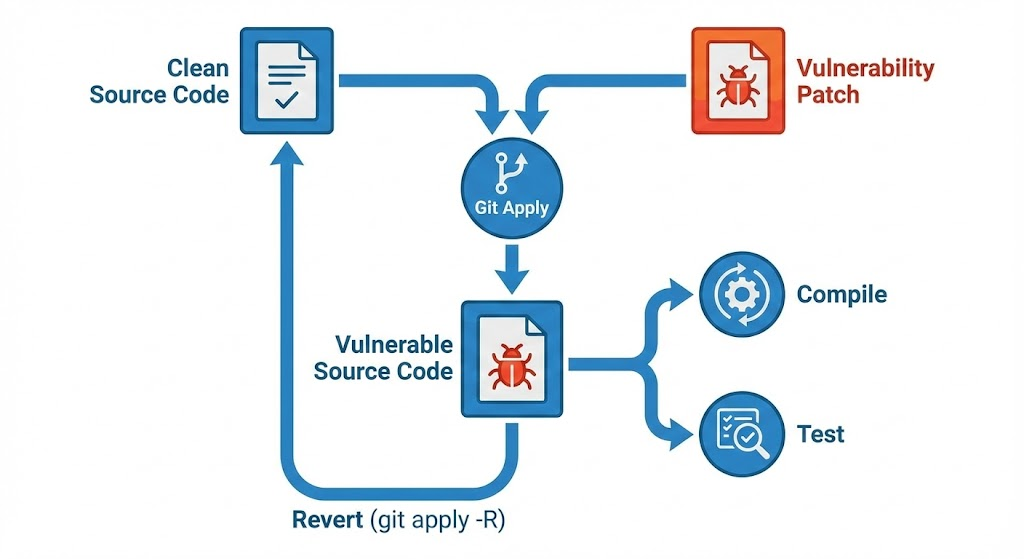
\includegraphics[width=0.75\textwidth]{resources/images/patch_lifecycle.jpg}
\caption{Patch Lifecycle: From vulnerability injection through evidence chain validation (diagram by author)}
\end{figure}

\section{Tools and Infrastructure}

\subsection{Compilation Toolchain}

The \textbf{compilation pipeline} begins with \textbf{clang}, which translates C code to \textbf{eBPF bytecode} suitable for kernel loading. Directly after compilation, we use \textbf{llvm-objdump} to inspect the compiled bytecode and confirm that \textbf{vulnerable code paths are present} and not optimized away by the compiler. A \textbf{Makefile} automates compilation steps and cleanup, ensuring \textbf{consistent build environment} and easy reproducibility.

\subsection{Kernel Tools}

Kernel interaction is mediated through several \textbf{essential tools}. The \textbf{bpftool} utility loads programs into the kernel, captures \textbf{verifier output} (including log files when requested), and dumps bytecode in multiple representations (xlated). The \textbf{trace\_pipe} interface provides access to kernel trace output, particularly \texttt{bpf\_printk} debug messages that PoC code can use to communicate status to user-space. The \textbf{ip link} command attaches and detaches XDP programs to specific network interfaces, a prerequisite for triggering execution.

\subsection{PoC Development}

Proof-of-concept code varies based on the vulnerability's nature. For simple network-based triggers, Python with the Scapy library provides high-level packet crafting. More intricate manipulation of packet structure, checksum recomputation, or ABI testing often requires raw socket programming in C. tcpdump is used for packet capture and inspection, confirming that PoC packets reach the kernel and observing the kernel's response.

\subsection{Test Environment}

All testing occurs in a \textbf{KVM/QEMU virtual machine} running \textbf{Linux LTS 6.8}, isolated from the host system. A \textbf{tmux} session manages multiple terminal panes simultaneously: one for kernel build and compilation, one for verifier interaction, one for trace output observation, and one for PoC execution. Simple tools like netcat assist in TCP-level testing when needed.

\section{Classification of Vulnerability Exploitability}

After executing the evidence chain, each vulnerability is classified into \textbf{one of three categories}, reflecting both the \textbf{verifier's acceptance} and the \textbf{exploitation potential} at runtime.

\subsection{Type-Safety Violation (Non-Corrupting)}

These vulnerabilities involve discrepancies between the verifier's type tracking and actual register contents, but do not result in memory corruption. The verifier accepts the program despite a type mismatch (e.g., treating a pointer as a scalar or vice versa), and the bytecode preserves this mismatch through verification. However, runtime behavior is observable but does not constitute memory corruption. A typical example is calling a kernel helper function with arguments of incorrect types; the call succeeds, but register values may be misaligned, leading to helper failures or unexpected returns rather than unsafe memory access.

\subsection{Exploitable (Memory Corruption Primitive)}

These vulnerabilities represent memory corruption primitives that enable concrete kernel attacks. The verifier fails to catch a bounds checking error, allowing the program at runtime to read or write beyond expected buffer boundaries. Such behavior can be chained into privilege escalation by writing to the process credentials structure, or information disclosure by reading kernel memory containing sensitive data. A typical example is a stack buffer overflow triggered via a tainted length parameter that the verifier failed to bound-check.

\subsection{Limited (Uncertain Exploitation)}

These vulnerabilities occupy a middle ground where the verifier accepts the program, evidence suggests a potential vulnerability, but exploitation feasibility is unclear without additional context or chaining with other primitives. A type confusion that might enable arbitrary pointer arithmetic but requires specific memory layout to trigger, or a bounds error that may not be reachable under normal execution patterns, fall into this category.

\section{Reproducibility and Validation}

\noindent
All findings are designed for \textbf{complete independent verification}. Patches are committed to version control with clear metadata describing the vulnerability injection. Compilation commands are recorded in Makefiles and can be executed identically on any machine with the same toolchain. Verifier logs, bytecode dumps, xlated bytecode, and artifact evidence are saved in structured directories under \texttt{src/exploits/<vulnerability-id>/logs/} for permanent reference and reproducibility. PoC scripts are documented with explicit trigger instructions and expected behavior.

To independently verify any finding, a reviewer needs only to \textbf{check out the same kernel version} (LTS 6.8), \textbf{apply the same patch} to the source (located in \texttt{XDPs/xdp\_synproxy/patches/}), \textbf{run the same compilation commands}, \textbf{attempt to load the program} using identical \texttt{bpftool} invocations, examine the saved artifact logs, and \textbf{execute the same PoC code} while observing runtime behavior. This \textbf{end-to-end reproducibility} is central to our methodology's credibility. All evidence artifacts are committed to the repository alongside the report.

\section{Infrastructure Modifications to Inherited Codebase}
\label{sec:infra-modifications}

The \textbf{previous team's infrastructure} provided a solid foundation but required \textbf{significant modifications and enhancements} to support practical exploitation with external-perspective attacks. This section documents all modifications made to their work to establish a functional testing environment.

\subsection{Virtual Machine Cloud-Init Configuration}

\begin{itemize}
\item \textbf{Files Modified}:
\begin{itemize}
  \item \texttt{virt/user-data.yaml} (cloud-init provisioning configuration)
\end{itemize}

\item \textbf{Status}: Created (file was missing from repository)

\item \textbf{Problem}: The previous team's \texttt{vmctl.sh} script referenced a cloud-init user-data file that was not included in the repository.

\item \textbf{Solution}: Created a comprehensive cloud-init configuration with: eBPF development tools (clang, llvm, bpftool), network utilities for testing (tcpdump, netcat, tshark, hping3), development tools (tmux, vim, git, make), kernel module loading support, and SSH key-based authentication.

\item \textbf{Impact}: Enabled automated VM provisioning with all required tools pre-installed and configured.
\end{itemize}

\subsection{Fixed SSH Key Substitution in VM Control Script}

\begin{itemize}
\item \textbf{Files Modified}:
\begin{itemize}
  \item \texttt{virt/vmctl.sh} (VM creation and provisioning automation)
\end{itemize}

\item \textbf{Status}: Modified (line ~51)

\item \textbf{Problem}: The original script used \texttt{sed} to substitute SSH public keys during provisioning, but SSH keys contain special characters (`/`, `+`, `=`, `\&`) that break \texttt{sed}'s delimiter-based pattern matching, causing the substitution to fail.

\item \textbf{Solution}: Replaced \texttt{sed} with \texttt{awk}, which handles variable substitution natively without requiring character escaping. The \texttt{awk} approach uses variable substitution and global replacement (\texttt{gsub}) to safely insert keys regardless of their character content.

\item \textbf{Impact}: VM provisioning now completes successfully regardless of SSH key format or special characters.
\end{itemize}

\subsection{Installed Host Virtualization Dependencies}

\begin{itemize}
\item \textbf{Location}: Host system (not part of inherited codebase)

\item \textbf{Status}: Prerequisite installation

\item \textbf{Problem}: Running \texttt{vmctl.sh create} failed because the virtualization tools (\texttt{virt-install}, \texttt{virtiofsd}, etc.) were not installed. The previous team's documentation assumed these would be present but did not account for Ubuntu 24.04's package naming conventions.

\item \textbf{Solution}: Installed the required virtualization packages: \texttt{virtinst}, \texttt{libvirt-daemon-system}, \texttt{libvirt-clients}, \texttt{qemu-system}, \texttt{qemu-utils}, and \texttt{virtiofsd}. Each package provides essential components for KVM/QEMU VM creation, management, and file sharing.

\item \textbf{Impact}: VM creation works on contemporary Ubuntu systems without manual package discovery and installation.
\end{itemize}

\subsection{Added Virtiofs Shared Folder Support}

\begin{itemize}
\item \textbf{Files Modified}:
\begin{itemize}
  \item \texttt{virt/vmctl.sh} (VM filesystem configuration)
  \item \texttt{virt/user-data.yaml} (shared folder auto-mount configuration)
\end{itemize}

\item \textbf{Status}: Enhanced

\item \textbf{Problem}: No mechanism existed to share files between host and VM. Docker is unsuitable for eBPF exploitation testing because it shares the host kernel. A dedicated VM with bidirectional file sharing enables editing code on the host while testing in an isolated kernel.

\item \textbf{Solution}: Added virtiofs filesystem support to the VM creation command and configured auto-mounting of the shared folder during cloud-init setup. This enables seamless host-to-VM file synchronization.

\item \textbf{Impact}: Host-to-VM file sharing enables seamless workflow: edit code on the host, test in the isolated VM kernel, and observe results without manual file transfer.
\end{itemize}

\subsection{Automated eBPF Compilation Environment Setup}

\begin{itemize}
\item \textbf{Files Modified}:
\begin{itemize}
  \item \texttt{virt/user-data.yaml} (cloud-init initialization commands)
  \item \texttt{XDPs/xdp\_synproxy/start\_session.sh} (automated test session setup)
\end{itemize}

\item \textbf{Status}: Enhanced

\item \textbf{Problem}: Manual setup of the eBPF compilation environment was required before each test, including extracting \texttt{vmlinux.h} from kernel BTF data, loading kernel modules, and creating necessary directories.

\item \textbf{Solution}: Automated the entire setup process by adding initialization commands to cloud-init configuration (executed during VM provisioning) and embedding setup logic in the test session script (executed when starting a test). Both approaches extract \texttt{vmlinux.h}, load required modules, and configure kernel parameters automatically.

\item \textbf{Impact}: The eBPF compilation environment is ready immediately after VM boot, eliminating manual setup steps before each test.
\end{itemize}

\subsection{Unified Path References and Workflow Clarity}

\begin{itemize}
\item \textbf{Files Modified}:
\begin{itemize}
  \item \texttt{XDPs/xdp\_synproxy/Makefile} (build automation)
  \item \texttt{XDPs/xdp\_synproxy/start\_session.sh} (test session setup)
  \item \texttt{README.md} (documentation and workflow guide)
\end{itemize}

\item \textbf{Status}: Consolidated

\item \textbf{Problem}: The inherited codebase used inconsistent path references relative to the \texttt{codebase/} subdirectory. When shared folders were introduced, these paths became ambiguous and contradicted the unified \texttt{/mnt/shared/} structure.

\item \textbf{Solution}: Modified all build scripts and documentation to consistently reference the shared folder mount point. Updated the Makefile to use unified paths, modified test session setup to point to the shared folder, and clarified the documentation with explicit patch application and test workflow instructions.

\item \textbf{Impact}: Consistent paths across host and VM eliminate navigation errors and clarify the exploitation workflow.
\end{itemize}

\subsection{Summary of Infrastructure Modifications}

\begin{table}[h]
\centering
\begin{tabular}{|l|l|l|}
\hline
\textbf{Component} & \textbf{Status} & \textbf{Benefit} \\
\hline
Cloud-init config & Created & Automated VM provisioning \\
SSH key handling & Fixed & Reliable key-based authentication \\
Host dependencies & Installed & Compatible virtualization stack \\
Shared folders & Added & Host-to-VM file synchronization \\
eBPF environment & Automated & Zero-manual-setup compilation \\
Path unification & Consolidated & Consistent workflow across tools \\
\hline
\end{tabular}
\caption{Summary of infrastructure modifications to inherited codebase}
\end{table}

These modifications transformed the inherited infrastructure from a theoretical testing framework into a practical, automated exploitation platform suitable for real-world vulnerability analysis and external-perspective attacks.
